\documentclass[10pt,a4paper,twoside,titlepage,twocolumn]{article}
\usepackage[utf8]{inputenc}
\usepackage[T1]{fontenc}
\usepackage[ngerman]{babel,varioref}
\usepackage[left=0.7cm,right=0.7cm,top=0.7cm,bottom=0.7cm,includeheadfoot]{geometry}

\usepackage{amsmath}
\usepackage{amssymb}
\usepackage{graphicx}
\usepackage{xcolor}
\usepackage{siunitx}



\begin{document}
    \graphicspath{ {./Images/} }


\definecolor{formulablue}{RGB}{219,219,255}
\newcommand{\formula}[1]{\colorbox{formulablue}{#1}}

\newcommand{\unitText}[3]{\noindent\textit{#1} : #2 [#3]}

\definecolor{refrot}{RGB}{183,28,42}
\newcommand{\refskript}[1]{\textcolor{refrot}{Skript S.#1}}



% \titlespacing*{\section}{0pt}{12pt}{0pt}
% \titlespacing*{\subsection}{0pt}{0pt}{0pt}
% \titlespacing*{\subsubsection}{0pt}{0pt}{0pt}


\title{\vspace{50mm}AdvDeLearn \\ [1ex] \large Summary}
\author{Lukas Schöpf}
% \titlepic{\vspace{50mm}\includegraphics[width=0.25\textwidth]{Elvis}}


% Code format
% Define the Gruvbox light colors
\definecolor{gruvbox_bg}{HTML}{fbf1c7}
\definecolor{gruvbox_fg}{HTML}{3c3836}
\definecolor{gruvbox_yellow}{HTML}{d79921}
\definecolor{gruvbox_red}{HTML}{cc241d}
\definecolor{gruvbox_green}{HTML}{98971a}
\definecolor{gruvbox_blue}{HTML}{458588}
\definecolor{gruvbox_purple}{HTML}{b16286}
\definecolor{gruvbox_aqua}{HTML}{689d6a}
\definecolor{gruvbox_orange}{HTML}{d65d0e}


% \lstdefinestyle{cppstyle}{
% 	language=C++,
% 	basicstyle=\ttfamily\footnotesize,
% 	numbers=left,
% 	numberstyle=\tiny,
% 	numbersep=5pt,
% 	tabsize=4,
% 	showspaces=false,
% 	showstringspaces=false,
% 	frame=single,
% 	rulecolor=\color{gruvbox_fg},
% 	backgroundcolor=\color{white},
% 	keywordstyle=\color{gruvbox_orange},
% 	commentstyle=\color{gruvbox_aqua},
% 	stringstyle=\color{gruvbox_green},
% 	identifierstyle=\color{gruvbox_fg},
% 	emphstyle=\color{gruvbox_red},
% 	emph={int, double, string, cout, TimerHandle_t, BaseType_t, timerPWMPeripheral_t, SemaphoreHandle_t, TaskHandle_t, QueueHandle_t},
% 	xleftmargin=5mm,
% 	xrightmargin=\parindent
% }

	\maketitle
	\setlength\parindent{0pt}

	% Uncomment these lines if you want to include the respective sections
	\section{Deep Learning Recap}

\subsection{Neural Network Types}
\subsubsection{Multi-Layer Perceptron (MLP)}
\begin{itemize}
    \item Input: \( n \)-dimensional, Output: \( m \)-dimensional.
    \item Fully connected hidden layers.
    \item Applications: Classification, regression, feature transformation, and dimensionality reduction.
\end{itemize}
Base equation / shallow network:
\[
f(x) = \sum_{i = 1}^{N} a_i \sigma(\mathbf{w}_i\cdot\mathbf{x} + b_i)
\]
For deep network:
\[
    y = f_3(f_2(f_1(x)))
\]

\subsubsection{Convolutional Neural Networks (CNNs)}
\begin{itemize}
    \item Feature extraction through convolutional layers.
    \item Supports multi-channel inputs (e.g., RGB images).
    \item Applications: Image processing, signal analysis, time-series data, 3D datasets like MRI.
\end{itemize}
Properties:
\begin{itemize}
    \item Weights(parameters) are shared
    \item Connections are sparse
    \item Each node in a layer has a receptive field
\end{itemize}
For multi-channel inputs, a diffrent kernel is applied for each channel.
The resulting channels are summed:
\[
C_{out,j} = b_j + \sum_{k=0}^{C_{in}-1} w \star f(x,y)
\]

Good practiec is to replace large filters with multiple smaller.

\subsection{Key Architectural Patterns}
\subsubsection{Reducing and Increasing Output Size}
\begin{itemize}
    \item Techniques: Strided convolutions, pooling, upsampling, and transposed convolutions.
\end{itemize}

\subsubsection{Improving Efficiency}
\begin{itemize}
    \item Bottleneck layers: Use \( 1 \times 1 \) convolutions to reduce channel dimensions.
    \item Separable filtes(for $7\times7$ use $(7\times1) \cdot (1\times7)$).
    \item Depthwise separable convolutions for sparse connectivity.
    \item Instead of one $11 \times 11$ conv. layer use 5 $3\times3$.
\end{itemize}

\subsubsection{Residual Connections}
\begin{itemize}
    \item Allow better gradient flow in deep networks.
    \item Key to ResNet architectures.
\end{itemize}

\subsubsection{Regularization}
\begin{itemize}
    \item Techniques: Dropout, \( L_2 \)-regularization.
    \item Goal: Prevent overfitting and improve generalization.
\end{itemize}

\subsection{Training Considerations}
\subsubsection{Layer/Batch normalization}
\begin{itemize}
    \item Use to normalize input to layers
    \item Accelerates training, importves generalization
\end{itemize}
\begin{equation*}
    \hat{x}^{(i)} = \frac{x^{(i)} - \mu_{\text{batch}}}{\sqrt{\sigma^2_{\text{batch}} + \epsilon}}
\end{equation*}
    
\begin{equation*}
    y^{(i)} = \gamma \hat{x}^{(i)} + \beta
\end{equation*}
\(\gamma\) and \(\beta\) are learnd from mini batches.

\subsubsection{Weight Initialization}
\begin{itemize}
    \item Xavier initialization ensures variance proportionality.
\end{itemize}

\subsubsection{Activation Functions}
\begin{itemize}
    \item Options: ReLU, Leaky ReLU, Sigmoid, Tanh, etc.
    \item ReLU variants preferred for stability.
\end{itemize}

\subsubsection{Optimizers}
\begin{itemize}
    \item Popular choices: SGD, Adam, RMSprop.
    \item Trade-offs between convergence speed and generalization.
\end{itemize}


	\section{Attention and Transformers}
\begin{figure}[ht]
    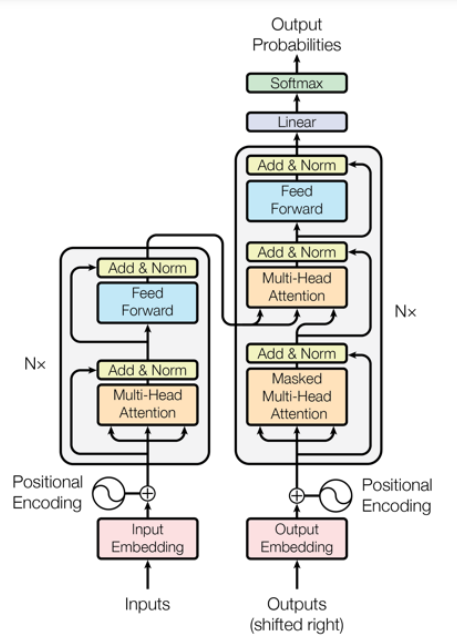
\includegraphics[width=0.6\columnwidth]{figures/AttentionTransformer/Transformer.png}
\end{figure}
\subsection{Sequence Processing}
\subsubsection{Recurrent Neural Networks (RNNs)}
\begin{itemize}
    \item Process sequences using recurrent cells with an internal state \( h \).
    \item Computation at each time step:
    \[
    h_t = \sigma(W_{hh} h_{t-1} + W_{xh} x_t + b_h)
    \]
    \item Output:
    \[
    y_t = W_{hy} h_t + b_y
    \]
    \item Common challenges: vanishing and exploding gradients.
\end{itemize}

\subsubsection{Advanced RNN Variants}
\begin{itemize}
    \item LSTMs handle long-term dependencies using gates:
    \[
    c_t = f_t \odot c_{t-1} + i_t \odot \tanh(W_c x_t + U_c h_{t-1} + b_c)
    \]
    \[
    h_t = o_t \odot \tanh(c_t)
    \]
    \item \(c_t\) long term memory
    \item \(h_t\) short term /working memory
    \item GRUs simplify LSTMs by merging the forget and input gates:
    \[
    h_t = (1 - z_t) \odot h_{t-1} + z_t \odot \tilde{h}_t
    \]
\end{itemize}
\begin{figure}
    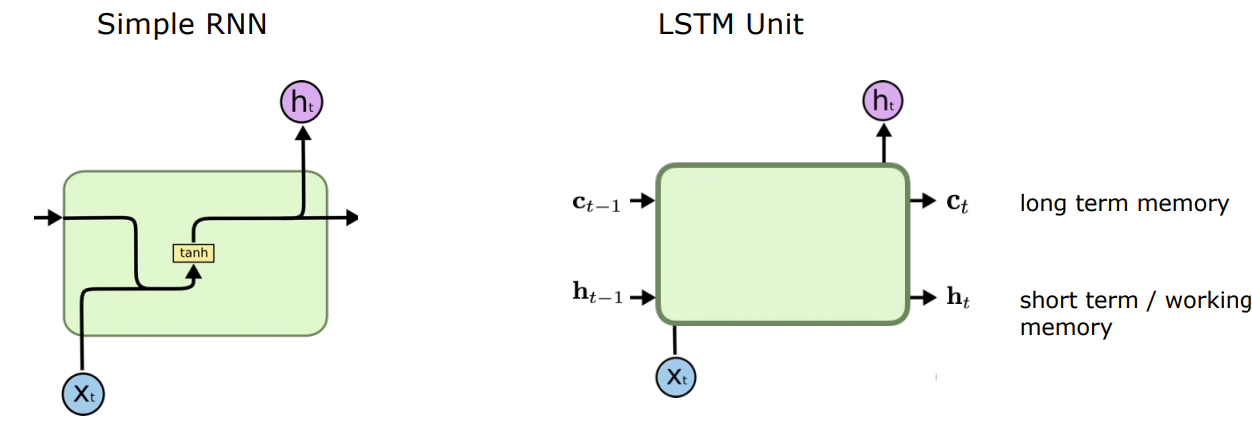
\includegraphics[width= \columnwidth]{figures/AttentionTransformer/RNNLSTM.png}
\end{figure}
\subsection{Attention Mechanism}
\subsubsection{Concept and Applications}
\begin{itemize}
    \item Attention aligns inputs with outputs for tasks like translation and image captioning.
    \item Improves handling of long sequences and offers interpretability.
\end{itemize}

\subsubsection{Attention Calculation}
\begin{itemize}
    \item Compute attention weights:
    \[
    \text{score}(q, k) = \frac{q \cdot k}{\sqrt{d_k}}
    \]
    \item Normalize weights with softmax:
    \[
    \alpha_{ij} = \frac{\exp(\text{score}(q_i, k_j))}{\sum_{j'} \exp(\text{score}(q_i, k_{j'}))}
    \]
    \item Compute the attention output as a weighted sum of values:
    \[
    \text{Attention}(Q, K, V) = \text{softmax}\left(\frac{QK^\top}{\sqrt{d_k}}\right)V
    \]
\end{itemize}

\subsection{Transformer Architecture}

\subsubsection{Encoder Architecture}
\begin{itemize}
    \item The encoder consists of \( N \) identical layers, each with:
    \begin{enumerate}
        \item Multi-head self-attention:
        \[
        \text{MultiHead}(Q, K, V) = \text{Concat}(\text{head}_1, \ldots, \text{head}_h)W^O
        \]
        where
        \[
        \text{head}_i = \text{Attention}(QW_i^Q, KW_i^K, VW_i^V)
        \]
        \item A feedforward network applied to each position:
        \[
        \text{FFN}(x) = \text{ReLU}(0, xW_1 + b_1)W_2 + b_2
        \]
        \item Residual connections and layer normalization for stability:
        \[
        \text{Output} = \text{LayerNorm}(x + \text{SubLayer}(x))
        \]
    \end{enumerate}
\end{itemize}

\subsubsection{Decoder Architecture}
\begin{itemize}
    \item The decoder mirrors the encoder but includes an additional sub-layer for cross-attention:
    \begin{enumerate}
        \item Masked multi-head self-attention:
        \[
        \text{Attention}(Q, K, V) = \text{softmax}\left(\frac{QK^\top}{\sqrt{d_k}}\right)V
        \]
        Masking prevents the decoder from seeing future tokens during training.
        \item Cross-attention, where queries come from the decoder, and keys/values come from the encoder.
        \item Feedforward network and residual connections (as in the encoder).
    \end{enumerate}
    \item A final linear layer projects the decoder's output to the vocabulary size, followed by a softmax:
    \[
    p(y_t | y_{<t}, x) = \text{softmax}(W_s h_t + b_s)
    \]
\end{itemize}

\subsubsection{Positional Encoding}
\begin{itemize}
    \item Adds sequence order information:
    \[
    PE_{\text{pos}, 2i} = \sin\left(\frac{\text{pos}}{10000^{2i/d_{\text{model}}}}\right)
    \]
    \[
    PE_{\text{pos}, 2i+1} = \cos\left(\frac{\text{pos}}{10000^{2i/d_{\text{model}}}}\right)
    \]
\end{itemize}
	\section{Vision Transformer (ViT)}
\begin{figure}[]
    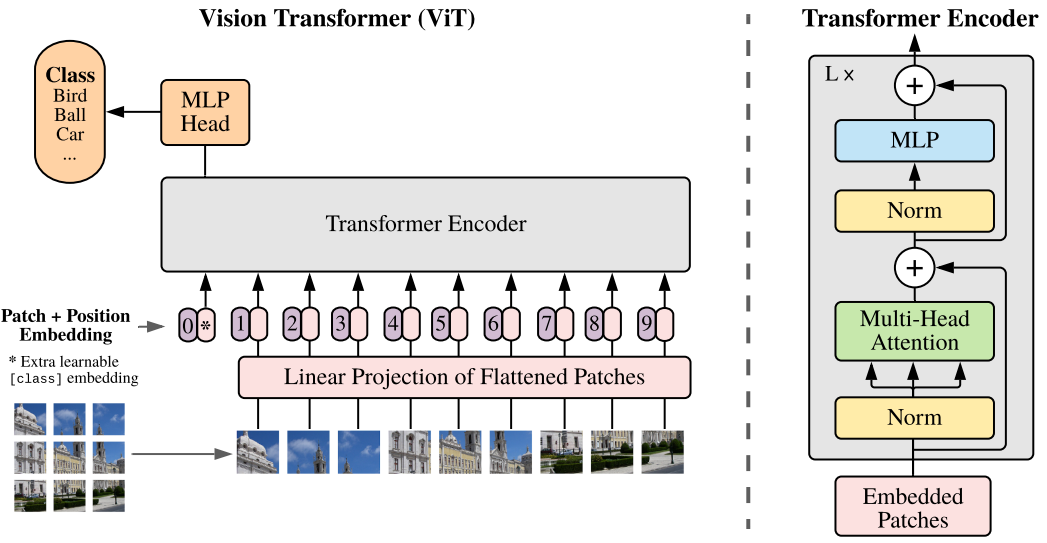
\includegraphics[width=\columnwidth]{figures/VisionTransformer/ViT.png}
\end{figure}
\begin{itemize}
    \item Extract square Images Patches
    \item Flatten Patches and project them to the embedding dimension D
    \item These embeddings are input to the Transformer
    \item Output of Transformer is fed into MLP or a singel layer
    \item Position embeddings added to input embeddings
\end{itemize}

Excellent results when pretrained on larger dataset(14M-300M)images and fine-tuned.

\subsection{Vertical Design}
\begin{figure}[!h]
    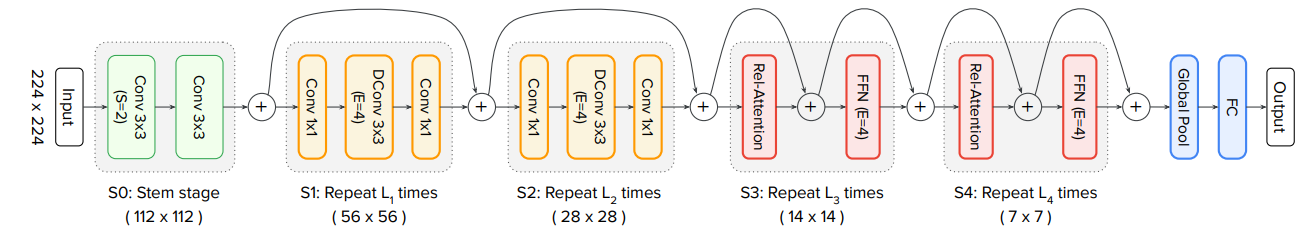
\includegraphics[width=\columnwidth]{figures/VisionTransformer/verticalDesign.png}
\end{figure}
\begin{itemize}
    \item Applying the relative-attention at pixel level is Computationally not possible
    \item A down-sampling of the image is needed
    \item Mimics CNNs architecture
\end{itemize}
\subsection{Relative self-Attention}
\begin{itemize}
    \item Combines Convolution and Attention
    \item Considers realitve position of tokens by introducing a global kernel value \(w_{i-j}\)
    \item  \textbf{Formula!}
\end{itemize}
	\section{Kolmogorov-Arnold Networks (KAN)}
The idea is to better approximate smooth functions with B-splines.

\subsection{B-Splines}
B-Splines are recursivly defined over a local area of knots(x coordinates)
Defined as \(B_{x-position,order}\).
\begin{figure}
    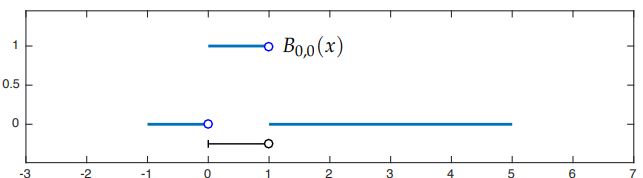
\includegraphics[width=0.5\columnwidth]{figures/KAN/BSplines1.png}
    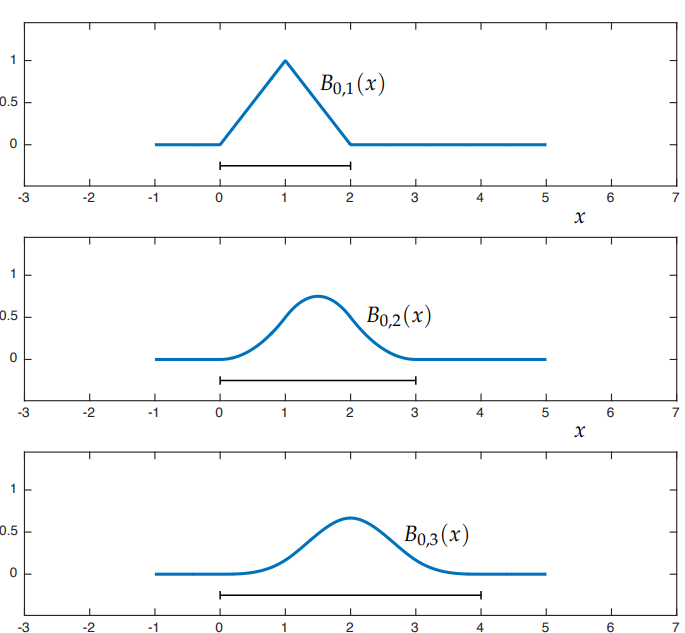
\includegraphics[width=0.5\columnwidth]{figures/KAN/BSplines2.png}
\end{figure}

\begin{figure}
    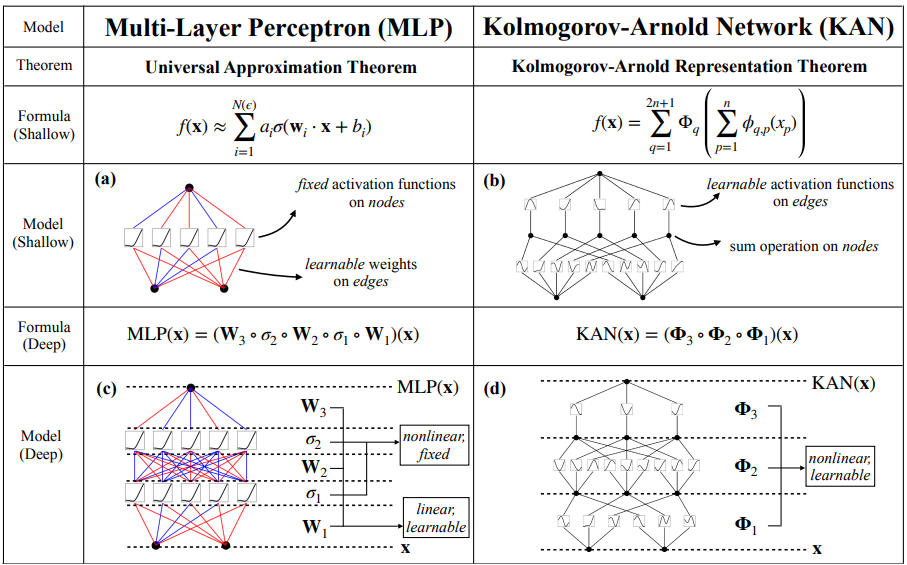
\includegraphics[width=\columnwidth]{figures/KAN/OverviewKANMLP.png}
\end{figure}
\begin{itemize}
    \item One main idea with the KANs is that they have better interpretability
    \item Aimed at math and physics applications
\end{itemize}
\subsection{Architecture}
\begin{itemize}
    \item Activation are on edges, not nodes, the nodes only do summation (no parameters)
    \item Non-linearity is applied on the edges before summing
\end{itemize}
	\section{Deep Reinforcement Learning}
\begin{figure}[!h]
    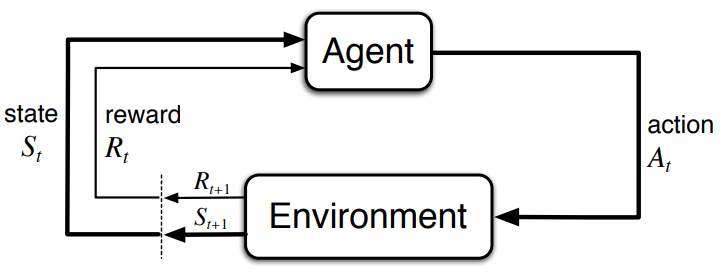
\includegraphics[width = 0.8\columnwidth]{figures/DeepReinforcementLearning/EnvironmentAgent.png}
\end{figure}

Agent learns from experience provided by a simulation of a environment.
The Goal is to maximize the expected cumulative reward/return.
cumulative reward or return (G):
\[
G_t = R_{t+1} + R_{t+2} + R_{t+3} + \dots + R_T
\]
Dicounted return:
\[
G_t = R_{t+1} + \gamma R_{t+2} +\gamma^2 R_{t+3} + \dots = \sum_{k=0}^{\infty}\gamma^k R_{t+k+1}
\]
\begin{figure}[!h]
    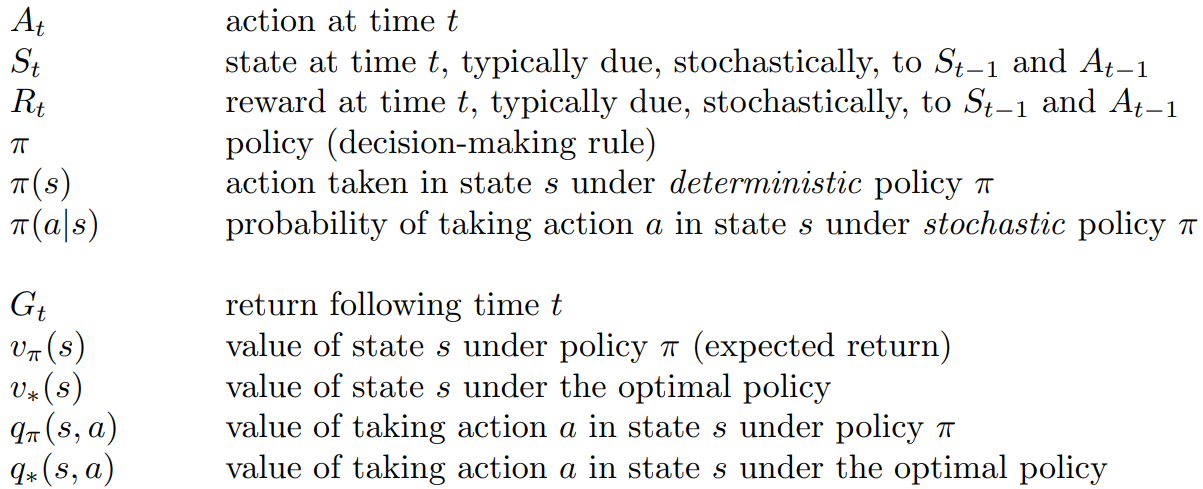
\includegraphics[width = \columnwidth]{figures/DeepReinforcementLearning/OverviewNotation.png}
\end{figure}
\subsection{Mehtods Overview}
\begin{figure}[!h]
    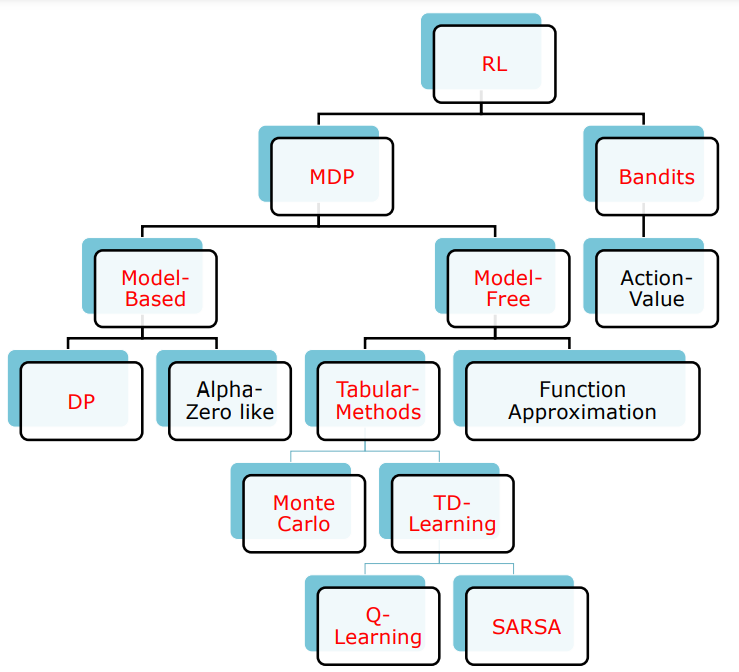
\includegraphics[width = \columnwidth]{figures/DeepReinforcementLearning/RLOverview.png}
\end{figure}
\subsubsection{Value based methods}
\begin{itemize}
    \item \textbf{Monte-Carlo Methods:} Estimate the returns from the rewards collected during the episode.Value estimation and policies are only changed \textbf{on the completion} of an episode

    \item \textbf{Time-Difference Methods:} Estimate the returns from the rewards and the approximated
    returns of the next step(s)
\end{itemize}
\begin{figure}[!h]
    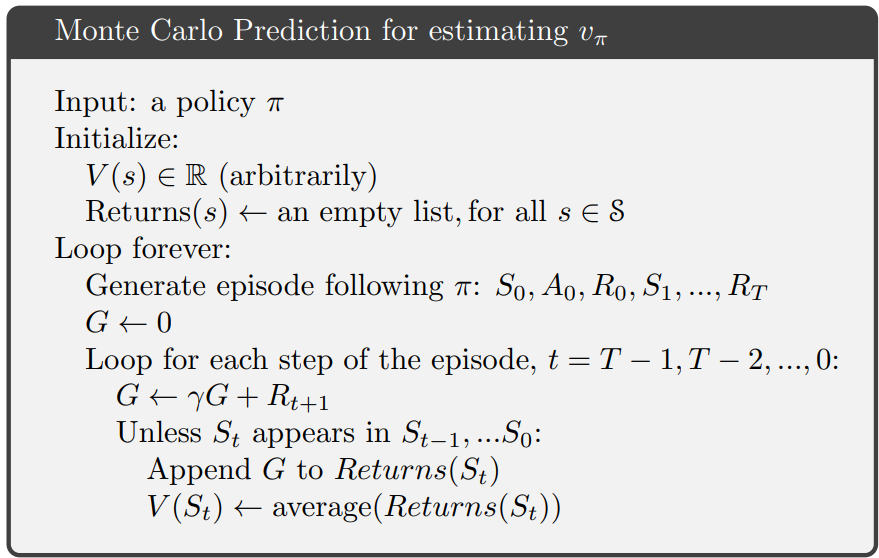
\includegraphics[width = \columnwidth]{figures/DeepReinforcementLearning/MonteCarlo.png}
\end{figure}



	% \input{Sections/04_Interprozesskommunikation}
	% \input{Sections/06_Deadlocks_PriorityInversion}
	% \input{Sections/07_Scheduling}
	% \input{Sections/08_Speicherhierarchie}
	% \input{Sections/10_Speicherverwaltung}
	
	% \input{Sections/99_CodeBeispiele}

\end{document}
